\documentclass[xcolor=x11names,compress]{beamer}

%\newcommand*{\upbullet}{\includegraphics[width=1em]{QC8_8.3_psi.pdf}}
%\setbeamertemplate{itemize item}{\upbullet}

%% General document %%%%%%%%%%%%%%%%%%%%%%%%%%%%%%%%%%
\usepackage{graphicx}
\usepackage{tikz}
\usetikzlibrary{decorations.fractals}
\usetikzlibrary{arrows,shapes}
\usetikzlibrary{shapes.geometric}
\usetikzlibrary{shadows}
\usetikzlibrary{snakes}
\usetikzlibrary{decorations.text}
\usepackage{fancybox}
\usepackage{amsmath}
\usepackage{graphics}
\usepackage[latin1]{inputenc}
\usefonttheme{professionalfonts}
\usepackage{times}
\usepackage{verbatim}
\usepackage{ragged2e}
\usepackage[justification=centering]{caption}
\usepackage{fancybox}
\usepackage{CJK}
\usepackage{media9}

%% Beamer Layout %%%%%%%%%%%%%%%%%%%%%%%%%%%%%%%%%%

\useoutertheme[subsection=false, shadow]{miniframes}
\useinnertheme{default}
\usefonttheme{serif}
\usepackage{palatino}

\setbeamercovered{transparent}  	%<<<<<----------------- This sets transparent itemized lists.
%\usefonttheme[onlymath]{serif}   	%<<<<<----------------- Sets the font only for formulas.

\setbeamerfont{title like}{shape=\scshape}
\setbeamerfont{frametitle}{shape=\scshape}

\setbeamercolor*{lower separation line head}{bg=DeepSkyBlue4} 
\setbeamercolor*{normal text}{fg=black,bg=white} 
\setbeamercolor*{alerted text}{fg=red} 
\setbeamercolor*{example text}{fg=black} 
\setbeamercolor*{structure}{fg=black} 
 
\setbeamercolor*{palette tertiary}{fg=black,bg=black!10} 
\setbeamercolor*{palette quaternary}{fg=black,bg=black!10} 

\renewcommand{\(}{\begin{columns}}
\renewcommand{\)}{\end{columns}}
\newcommand{\<}[1]{\begin{column}{#1}}
\renewcommand{\>}{\end{column}}
\setbeamertemplate{navigation symbols}{}

%\setbeamertemplate{footline}[page number]
\setbeamertemplate{footline}
{
  \leavevmode%
  \hbox{%
  \begin{beamercolorbox}[wd=.28\paperwidth,ht=2.25ex,dp=1ex,center]{author in head/foot}%
    \usebeamerfont{author in head/foot}Joseph M. Fedrow  \end{beamercolorbox}%
  \begin{beamercolorbox}[wd=.44\paperwidth,ht=2.25ex,dp=1ex,center]{title in head/foot}%
    \usebeamerfont{title in head/foot}Git and LaTeX for Your Scientific Workflow \end{beamercolorbox}%
  \begin{beamercolorbox}[wd=.28\paperwidth,ht=2.25ex,dp=1ex,right]{date in head/foot}%
    \usebeamerfont{date in head/foot}\insertshortdate{}\hspace*{2em}
    \insertframenumber{} / \inserttotalframenumber\hspace*{2ex} 
  \end{beamercolorbox}}%
  \vskip0pt%
}


%%%%%%%%%%%%%%%%%%%%%%%%%%%%%%%%%%%%%%%%%%%%%%%%%%%%%%
%
%
\begin{document} 

\section{\scshape Introduction}
\subsection{Introduction}

\begin{frame}
\vspace{-0.5cm}
\title{
Git Your \LaTeX\,On!
}\author{
	Joseph M. Fedrow\\
	\vspace{0.5cm}
	\begin{tikzpicture}[decoration=Koch snowflake]
		\draw[DeepSkyBlue4] decorate{ decorate{ decorate{ (0,0) -- (3,0) }}};
	\end{tikzpicture}
	\vspace{-0.8cm}
}

\date{
	\today
	}
	
	\titlepage
	`
	\vspace{-0.5cm}
	
	
	
	 \centerline{
\includegraphics[scale=0.3]{asu-logo-E9CC4BDF34-seeklogo.com} \hspace{1.115cm}  
\includegraphics[scale=0.18]{asu-logo-DA1C895AD3-seeklogo.com}  \hfill{} 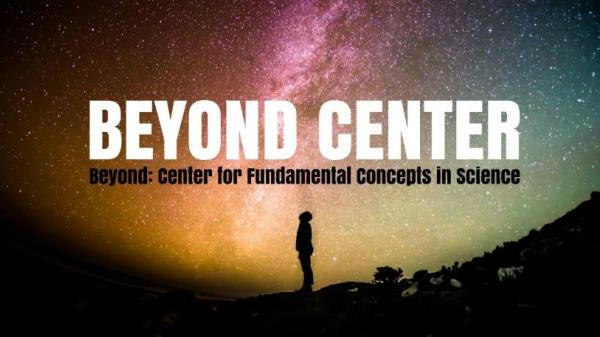
\includegraphics[scale=0.19]{Beyond Center Logo (New)}}

\end{frame}

\frame{
\frametitle{What is Git and LaTeX?}


\centerline{
\includegraphics[scale=0.2]{1}} 

\vfill

\centerline{Version control and Typesetting}

}

\frame{
\frametitle{How Can They Help You?}

Version Control:\\

The practice of tracking and managing changes to source code over time\\

Keeps track of every modification to the code in a special kind of database. If a mistake is made, developers can turn back the clock and compare earlier versions of the code

Good for backups and making non-destructive edits\\ 

Really shines when working in teams on collaborative projects.\\

\centerline{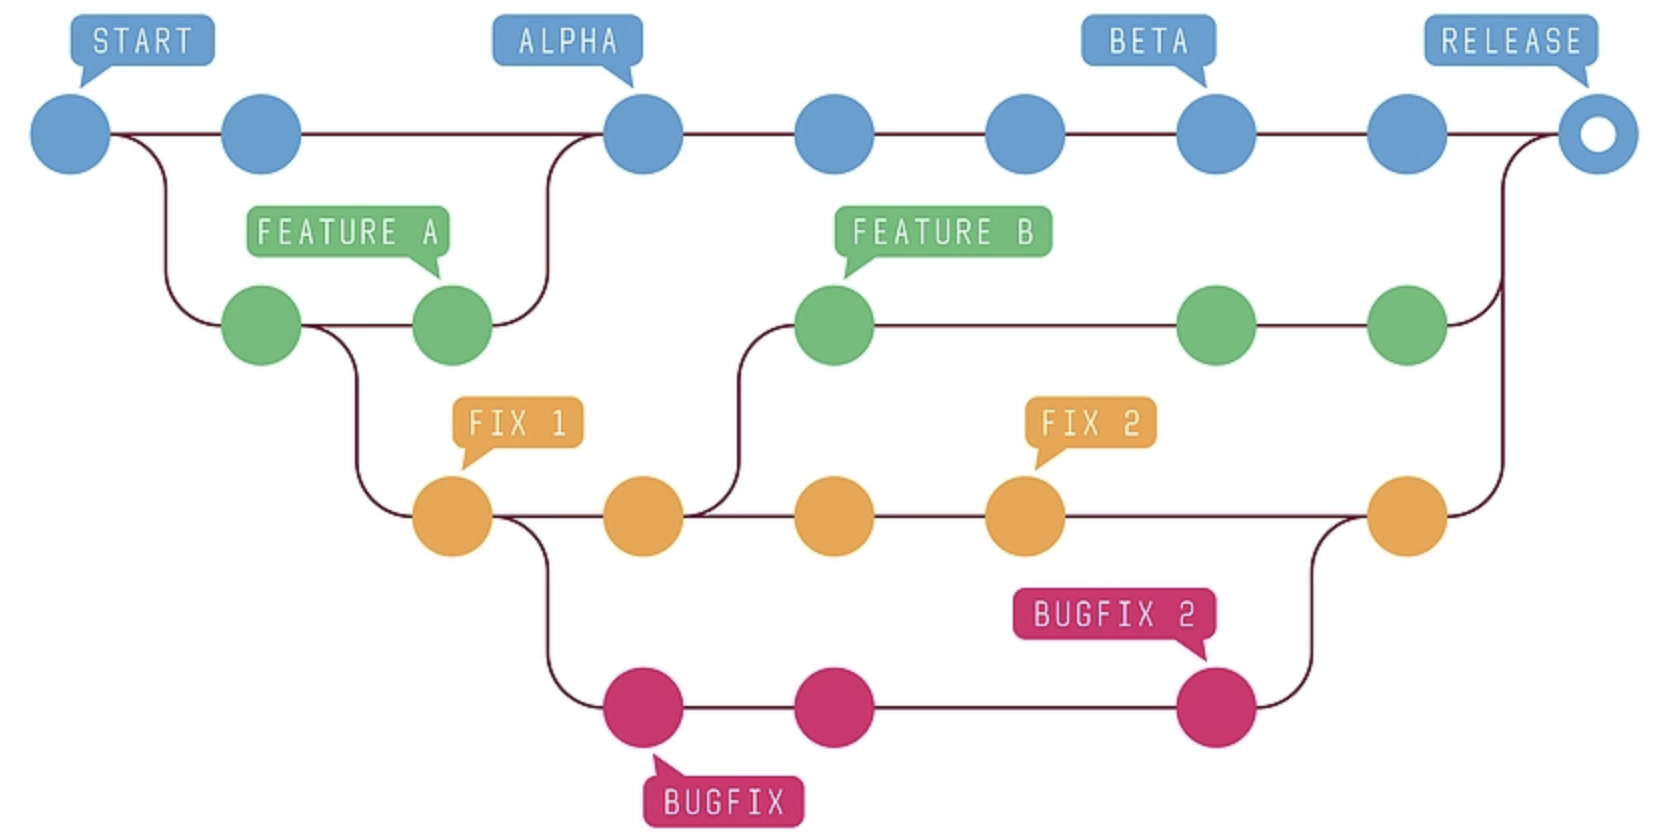
\includegraphics[scale=0.25]{3}} 

}

\frame{
\frametitle{How Can They Help You?}

Typesetting:\\ 

Helps make your documents looks professional.\\ 

Really shines when working with equations and tables.\\

 \centerline{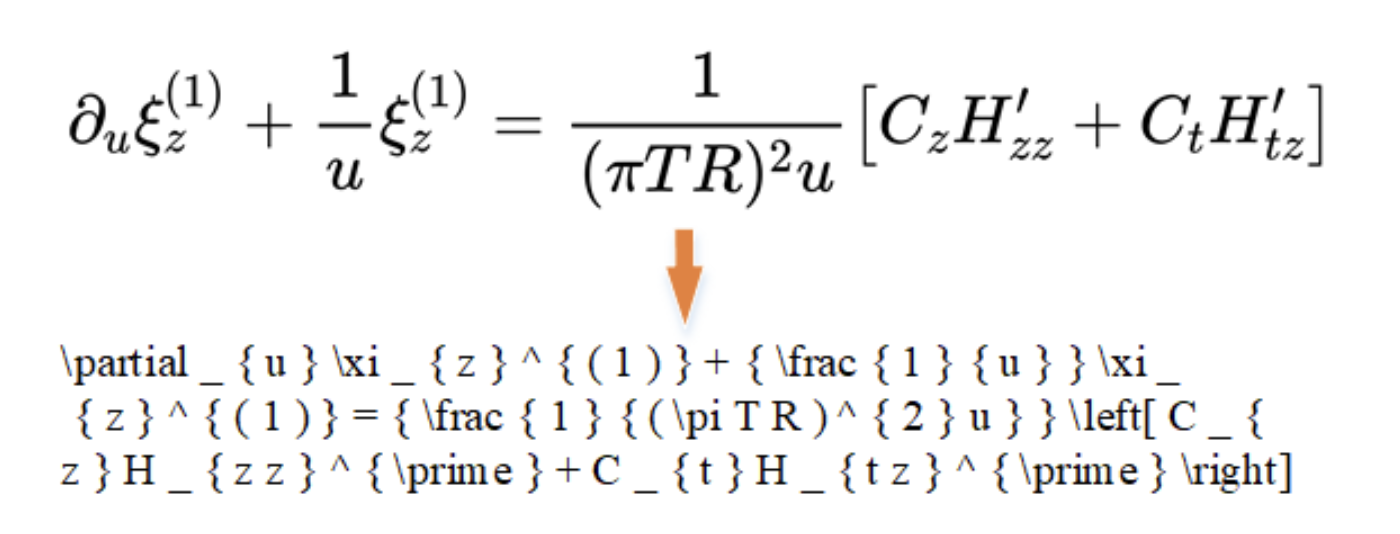
\includegraphics[scale=0.42]{4}} 

}


\section{\scshape Git}
\subsection{Git}

\frame{
\frametitle{History and Philosophy of Git}

2002: BitKeeper for Linux (propietary) \\

2005: Git \\

Git is free and open source \\

\textit{Distributed} Version Control System (DVCS)\\
Every clone is really a full backup of all the data.\\


}

\frame{
\frametitle{Git is not Github!}

\centerline{Git is a piece of software. GitHub is an online SaaS service.}

\centerline{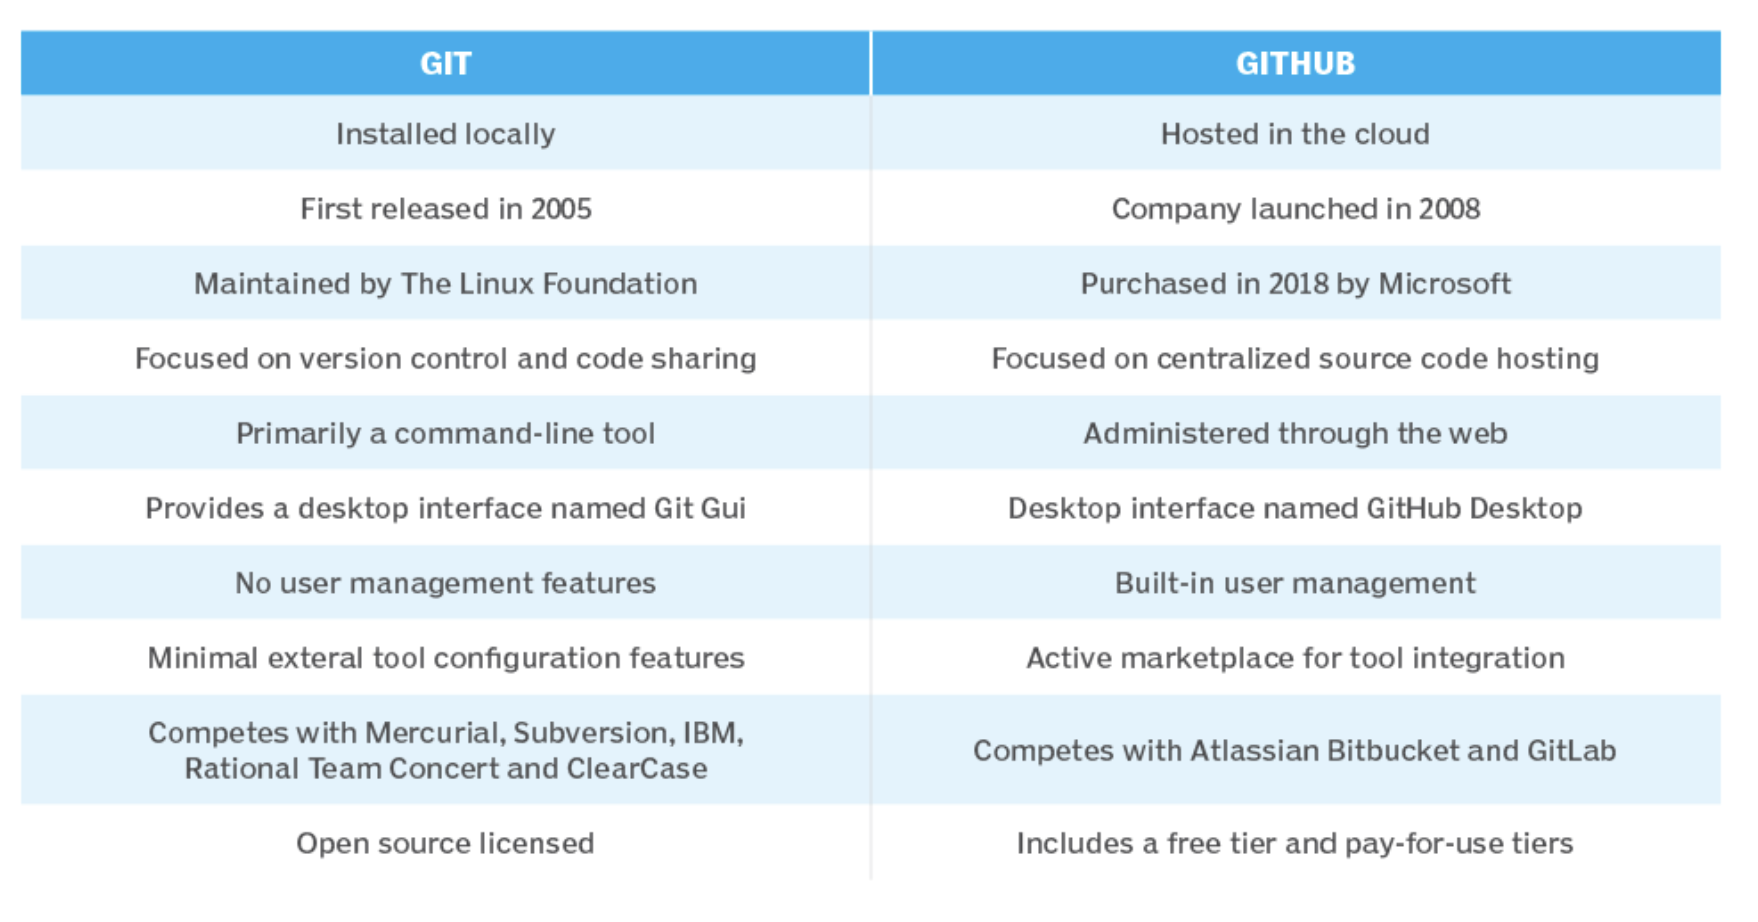
\includegraphics[scale=0.4]{2}} 

}


\frame{
\frametitle{How to Use Git}

Install: git --version (osx)\\


https://git-scm.com/book/en/v2/Getting-Started-Installing-Git

}

\frame{
\frametitle{When diving into Git...}

\centerline{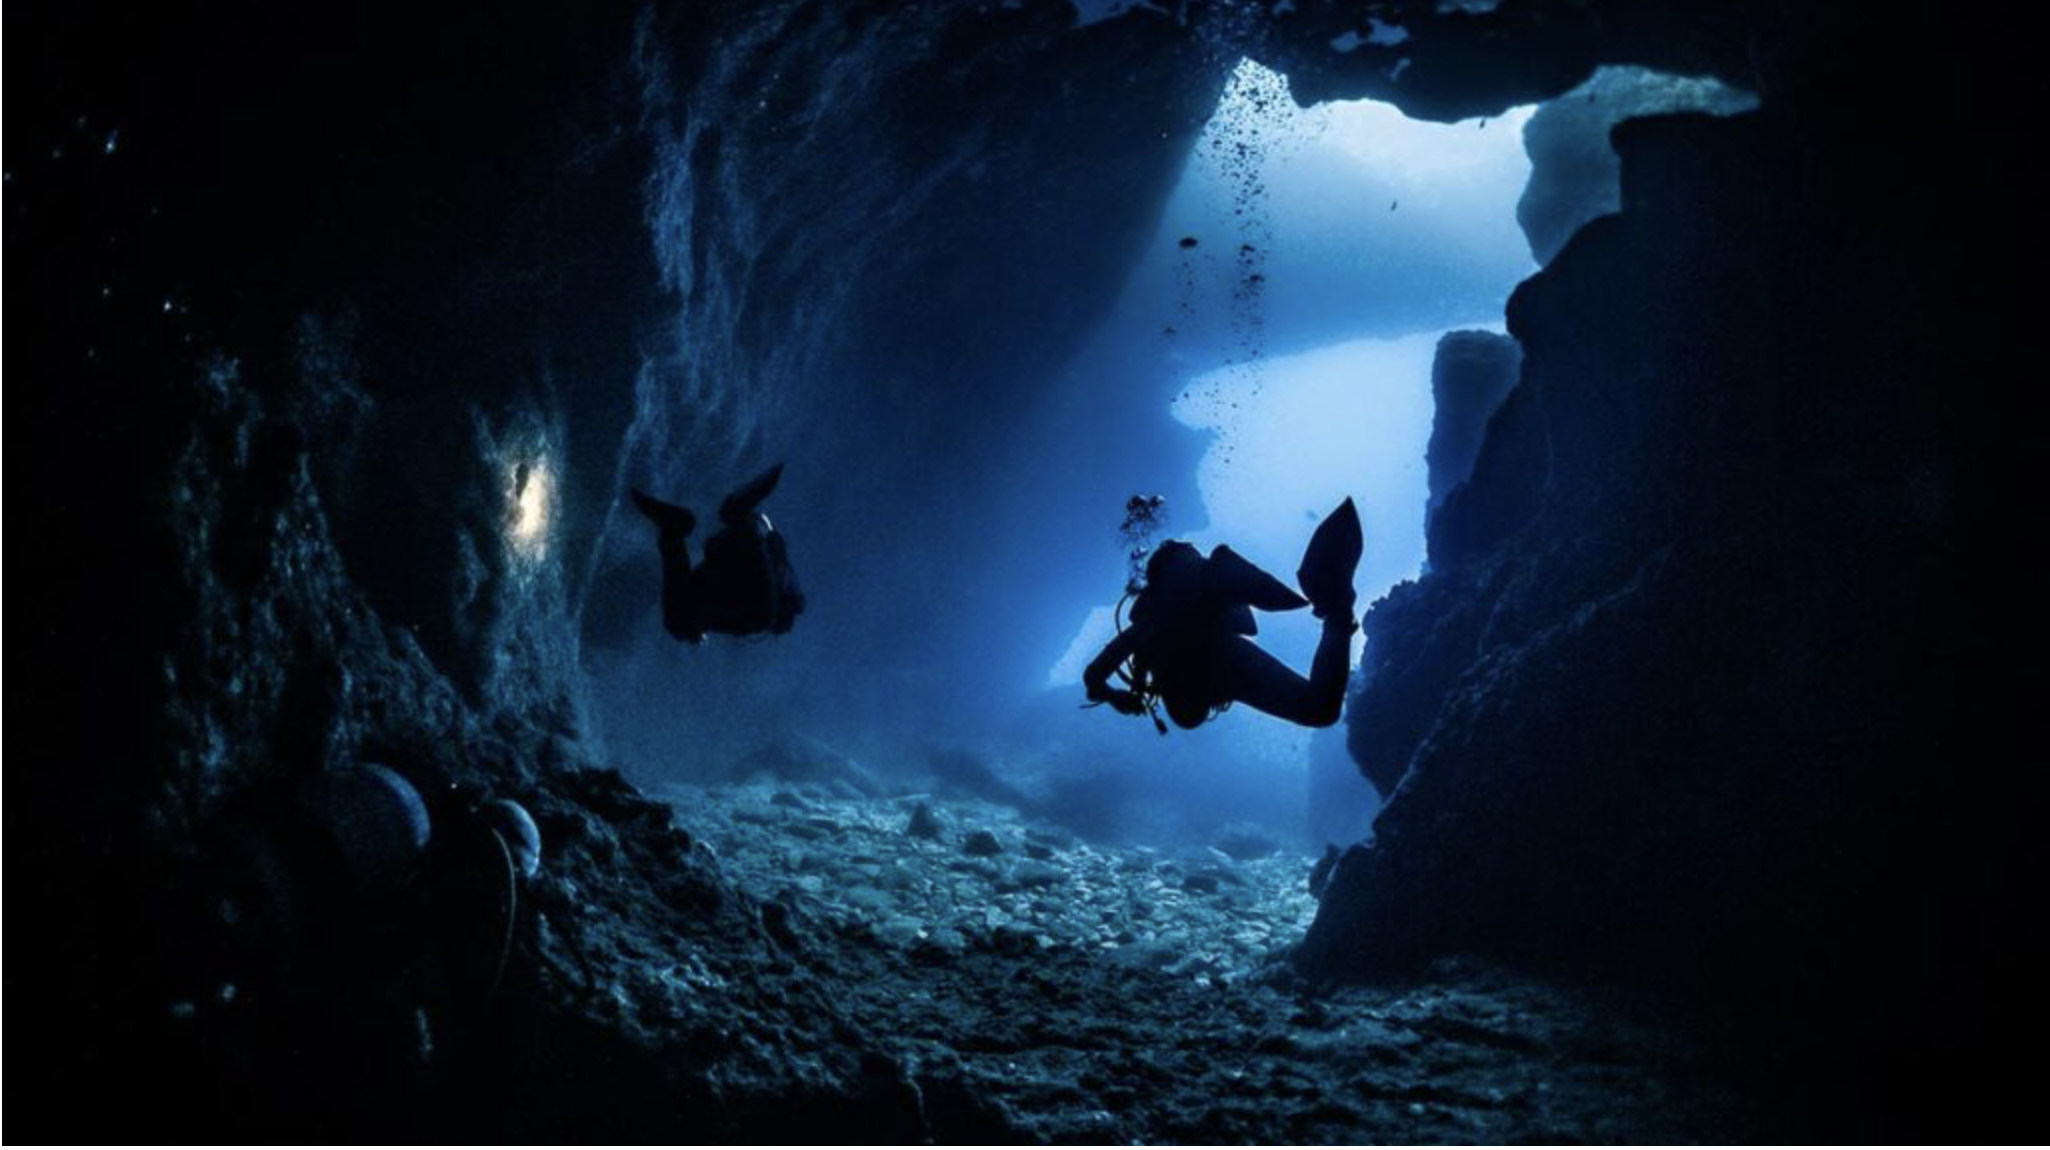
\includegraphics[scale=0.32]{5}} 

}

\frame{
\frametitle{Your path can be simple...}


\centerline{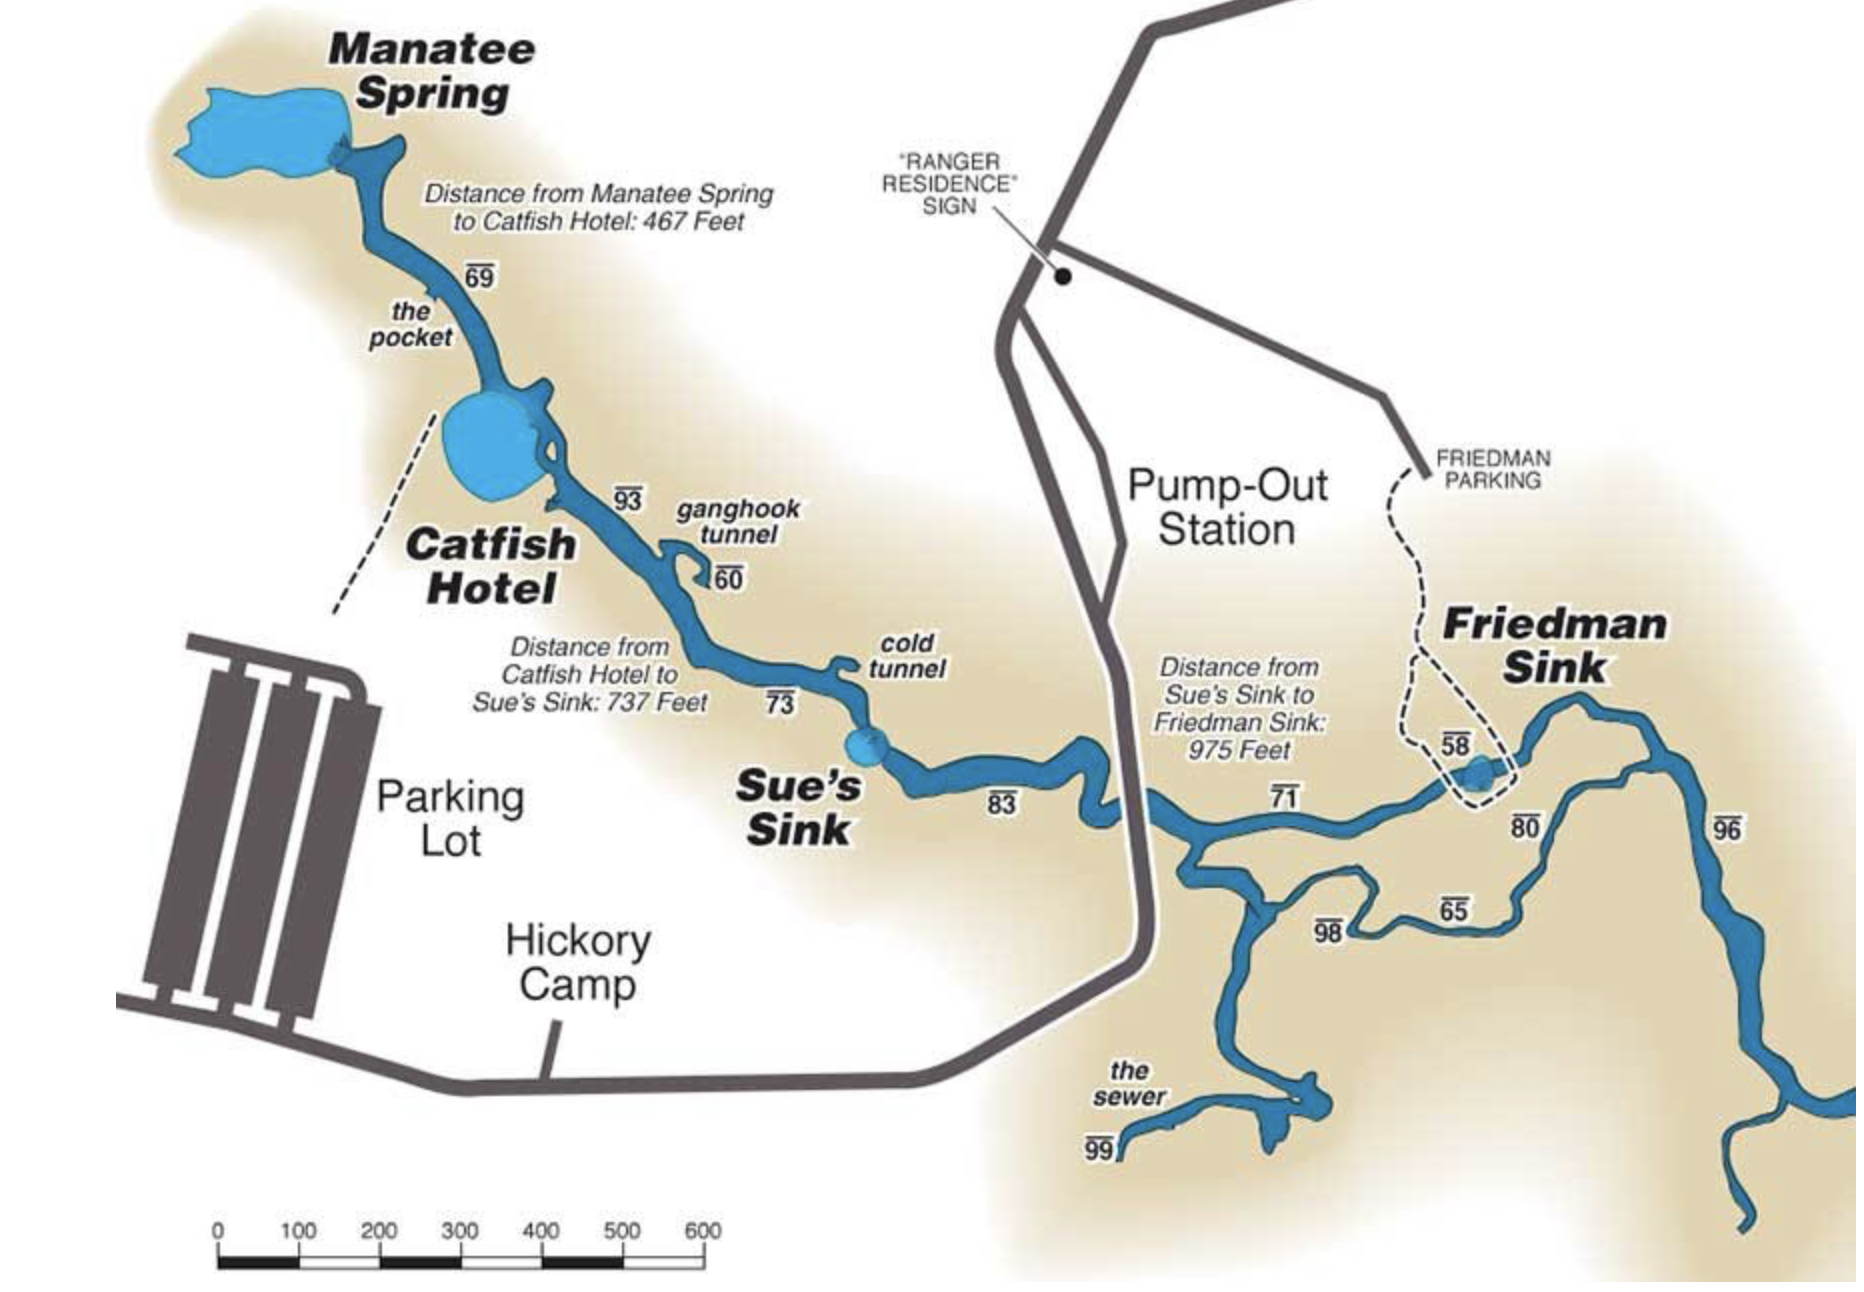
\includegraphics[scale=0.28]{6}} 

}

\frame{
\frametitle{Or as complicated as you like.}

\centerline{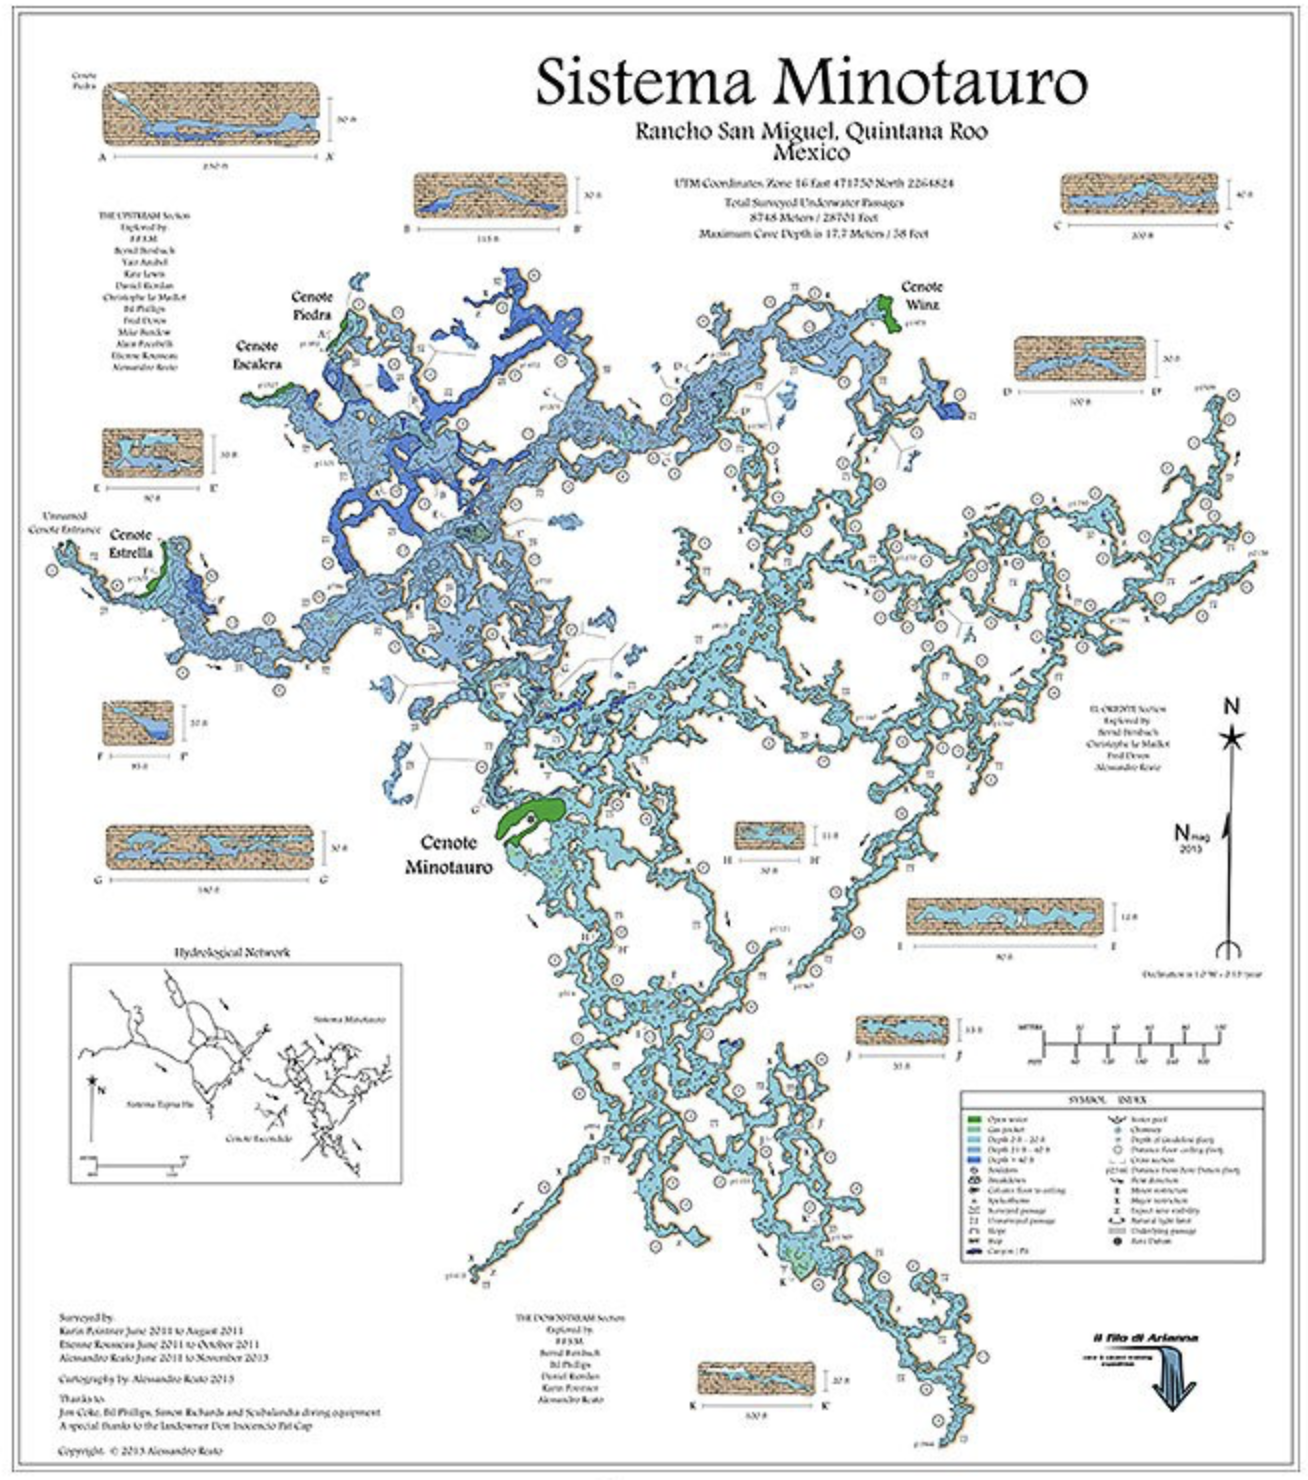
\includegraphics[scale=0.28]{7}} 

}




\section{\scshape LaTeX}
\subsection{LaTeX}


\frame{
\frametitle{History of Tex and LaTeX}

1977 Donald Knuth developed Tex-- a computer language and program designed for use in typesetting; in particular, for typesetting math and other technical (from Greek "techne" = art/craft, the stem of `technology') material. \\

LaTeX was originally written in the early 1980s by Leslie Lamport at SRI International\\

LaTeX is intended to provide a high-level, descriptive markup language to utilize TeX more easily. TeX handles the document layout, while LaTeX handles the content side for document processing.\\


}

\frame{
\frametitle{How to Use LaTeX}

This write-format-preview cycle is one of the chief ways in which working with LaTeX differs from the What-You-See-Is-What-You-Get (WYSIWYG) style of document editing. It is similar to the code-compile-execute cycle known to computer programmers. 

}

\section{\scshape Surprise!}
\subsection{Surprise!}

\frame{
\frametitle{This Entire Presentation Was Done\\ in Git and \LaTeX !}

}

\section{\scshape Summary}
\subsection{Summary}

\frame{
\frametitle{Summary}

}

\frame{
\frametitle{Resources}

https://git-scm.com/book/en/v2

}

\end{document}


